\documentclass{standalone}
\usepackage{tikz}  % package pour les graphes
\usetikzlibrary{positioning,shapes,arrows}
\usetikzlibrary{bayesnet}

\begin{document}
	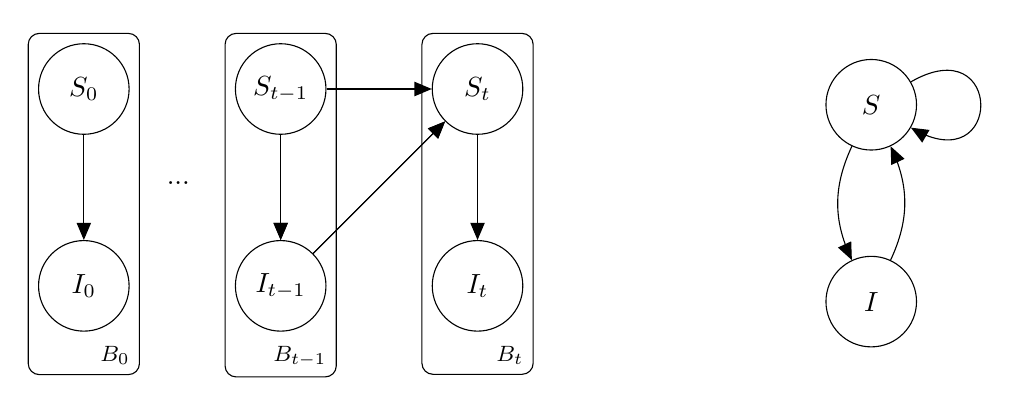
\begin{tikzpicture}[node distance={25mm}, main/.style = {draw, circle, minimum size=1.15cm}]
	\node[main] (S0) {$S_0$};
	\node[main] (I0) [below of=S0] {$I_0$};
	\node (L) at (1.2, -1.2) {...};
	\node[main] (S1) [right of=S0]{$S_{t-1}$};
	\node[main] (I1) [below of=S1] {$I_{t-1}$};
	\node[main] (S2) [right of=S1] {$S_{t}$};
	\node[main] (I2) [below of=S2] {$I_{t}$};

	\node[main] (S) at (10, -0.2) {$S$};
	\node[main] (I) [below of=S] {$I$};

	
	\draw[->] (S0) -- (I0);
	\draw[->] (S1) -- (I1);
	\draw[->] (S1) -- (S2);
	\draw[->] (I1) -- (S2);
	\draw[->] (I1) -- (S2);
	\draw[->] (S1) -- (I1);
	\draw[->] (S2) -- (I2);
	
	\draw[->] (S) edge[bend right=25] (I);
	\draw[->] (I) edge[bend right=25] (S);
	\draw[->] (S) to[out=30, in=-30, looseness=6] (S);	
	
	% Plates
	\plate {A} {(S0)(I0)} {$B_0$} ;
	\plate {B} {(S1)(I1)} {$B_{t-1}$} ;
	\plate {C} {(S2)(I2)} {$B_t$} ;
	
	
\end{tikzpicture}
\end{document}